%%%%%%%%%%%%%%%%%%%%%%%%%%%%%%%%%%%%%%%%%%%%%%%%%%%%%%%%%%%%%%%%%%%%%%%%%%%%%%%
% CASE STUDY TEMPLATE - Programming and Problem Solving
% Author: Brendan Shea, PhD
% Course: Programming and Problem Solving
% Rochester Community and Technical College
%%%%%%%%%%%%%%%%%%%%%%%%%%%%%%%%%%%%%%%%%%%%%%%%%%%%%%%%%%%%%%%%%%%%%%%%%%%%%%%

\documentclass[11pt,letterpaper]{article}

%---------- PACKAGES ----------%
\usepackage[margin=1in, headheight=22pt]{geometry}
\usepackage[T1]{fontenc}
\usepackage{xcolor}
\usepackage{tcolorbox}
\usepackage{graphicx}
\usepackage{titlesec}
\usepackage{enumitem}
\usepackage{fancyhdr}
\usepackage{listings}
\usepackage{hyperref}
\usepackage{multicol}
\usepackage{booktabs}
\usepackage{tikz}
\usepackage{float}
\usepackage{amssymb}
\usepackage{amsmath}
\usepackage{pifont}

% TikZ libraries
\usetikzlibrary{shapes.geometric, arrows.meta, positioning, calc, backgrounds, fit, matrix, decorations.pathreplacing, chains}

% Load tcolorbox libraries
\tcbuselibrary{skins,breakable,listings,listingsutf8}

%---------- COLOR DEFINITIONS ----------%
\definecolor{csprimary}{HTML}{2C3E50}
\definecolor{cssecondary}{HTML}{E74C3C}
\definecolor{cstertiary}{HTML}{3498DB}
\definecolor{csaccent}{HTML}{27AE60}
\definecolor{cswarm}{HTML}{F39C12}
\definecolor{cslight}{HTML}{ECF0F1}
\definecolor{csdark}{HTML}{1A252F}

% Syntax highlighting colors
\definecolor{codegreen}{HTML}{27AE60}
\definecolor{codepurple}{HTML}{9B59B6}
\definecolor{codeorange}{HTML}{E67E22}
\definecolor{codeblue}{HTML}{3498DB}
\definecolor{codegray}{HTML}{95A5A6}
\definecolor{codestring}{HTML}{E74C3C}
\definecolor{codebg}{HTML}{1E2A38}

%---------- CASE STUDY METADATA ----------%
\newcommand{\cstitle}{Pixels to Polygons}
\newcommand{\cssubtitle}{A Short History of Video Game Programming}
\newcommand{\csauthor}{Brendan Shea, PhD}
\newcommand{\cscourse}{Programming and Problem Solving}
\newcommand{\csinstitution}{Rochester Community and Technical College}
\newcommand{\csdate}{\today}

%---------- LISTINGS CONFIGURATION ----------%
\lstdefinestyle{basestyle}{
    backgroundcolor=\color{codebg},
    basicstyle=\ttfamily\small\color{white},
    breakatwhitespace=false,
    breaklines=true,
    captionpos=b,
    keepspaces=true,
    showspaces=false,
    showstringspaces=false,
    showtabs=false,
    tabsize=4,
    frame=none,
    xleftmargin=4mm,
    xrightmargin=4mm,
    aboveskip=0pt,
    belowskip=0pt,
}

\lstdefinestyle{javastyle}{
    style=basestyle,
    language=Java,
    keywordstyle=\color{codeblue}\bfseries,
    commentstyle=\color{codegray}\itshape,
    stringstyle=\color{codestring},
    morekeywords={String, Scanner, System, var, boolean, Math, List, Map,
                  HashMap, ArrayList, enum, interface, abstract, override},
}

\lstdefinestyle{asmstyle}{
    style=basestyle,
    keywordstyle=\color{codeblue}\bfseries,
    commentstyle=\color{codegray}\itshape,
    morekeywords={LDA, STA, LDX, STX, LDY, STY, CMP, BEQ, BNE, BCC, BCS,
                  JMP, JSR, RTS, INC, DEC, AND, ORA, EOR, ASL, LSR, PHA, PLA},
}

%---------- CUSTOM ENVIRONMENTS ----------%
\newcommand{\keyterm}[1]{\textbf{\textcolor{cssecondary}{#1}}}

\newtcolorbox{conceptbox}[1][]{
    enhanced,
    colback=cslight,
    colframe=csprimary,
    fonttitle=\bfseries\color{white},
    title=#1,
    attach boxed title to top left={yshift=-2mm, xshift=5mm},
    boxed title style={colback=csprimary},
    breakable
}

\newtcolorbox{historybox}[1][]{
    enhanced,
    colback=codepurple!8,
    colframe=codepurple,
    fonttitle=\bfseries\color{white},
    title=#1,
    attach boxed title to top left={yshift=-2mm, xshift=5mm},
    boxed title style={colback=codepurple},
    breakable
}

\newtcolorbox{tipbox}[1][]{
    enhanced,
    colback=csaccent!8,
    colframe=csaccent,
    fonttitle=\bfseries\color{white},
    title=#1,
    attach boxed title to top left={yshift=-2mm, xshift=5mm},
    boxed title style={colback=csaccent},
    breakable
}

\newtcolorbox{debatebox}[1][]{
    enhanced,
    colback=cswarm!8,
    colframe=cswarm,
    fonttitle=\bfseries\color{white},
    title=#1,
    attach boxed title to top left={yshift=-2mm, xshift=5mm},
    boxed title style={colback=cswarm},
    breakable
}

\newtcolorbox{quotebox}[1][]{
    enhanced,
    colback=cstertiary!8,
    colframe=cstertiary,
    fonttitle=\bfseries\color{white},
    title=#1,
    attach boxed title to top left={yshift=-2mm, xshift=5mm},
    boxed title style={colback=cstertiary},
    breakable
}

\newtcblisting{javacode}[1][]{
    enhanced,
    colback=codebg,
    colframe=csaccent,
    colupper=white,
    fonttitle=\bfseries\color{white},
    title=#1,
    attach boxed title to top left={yshift=-2mm, xshift=5mm},
    boxed title style={colback=csaccent},
    left=0mm, right=0mm, top=2mm, bottom=2mm,
    boxrule=1pt,
    breakable,
    pad at break=2mm,
    listing only,
    listing options={style=javastyle}
}

\newtcblisting{asmcode}[1][]{
    enhanced,
    colback=codebg,
    colframe=cssecondary,
    colupper=white,
    fonttitle=\bfseries\color{white},
    title=#1,
    attach boxed title to top left={yshift=-2mm, xshift=5mm},
    boxed title style={colback=cssecondary},
    left=0mm, right=0mm, top=2mm, bottom=2mm,
    boxrule=1pt,
    breakable,
    pad at break=2mm,
    listing only,
    listing options={style=asmstyle}
}

\newtcolorbox{questionbox}{
    enhanced,
    colback=cswarm!10,
    colframe=cswarm,
    fonttitle=\bfseries\color{white},
    title=Discussion Questions,
    attach boxed title to top center={yshift=-2mm},
    boxed title style={colback=cswarm},
    breakable
}

\newtcolorbox{glossarybox}{
    enhanced,
    colback=cslight,
    colframe=csprimary,
    fonttitle=\bfseries\color{white},
    title=Glossary of Key Terms,
    attach boxed title to top center={yshift=-2mm},
    boxed title style={colback=csprimary},
    breakable
}

%---------- HEADER/FOOTER ----------%
\pagestyle{fancy}
\fancyhf{}
\fancyhead[L]{\small\textcolor{csprimary}{\cscourse}}
\fancyhead[R]{\small\textcolor{csprimary}{Case Study}}
\fancyfoot[C]{\thepage}
\renewcommand{\headrulewidth}{0.4pt}
\renewcommand{\headrule}{\hbox to\headwidth{\color{csprimary}\leaders\hrule height \headrulewidth\hfill}}

%---------- SECTION FORMATTING ----------%
\titleformat{\section}
    {\Large\bfseries\color{csprimary}}
    {\thesection}{1em}{}[\color{cssecondary}\titlerule]

\titleformat{\subsection}
    {\large\bfseries\color{cstertiary}}
    {\thesubsection}{1em}{}

%---------- HYPERLINK SETTINGS ----------%
\hypersetup{
    colorlinks=true,
    linkcolor=cstertiary,
    urlcolor=cstertiary
}

%%%%%%%%%%%%%%%%%%%%%%%%%%%%%%%%%%%%%%%%%%%%%%%%%%%%%%%%%%%%%%%%%%%%%%%%%%%%%%%
\begin{document}

%---------- TITLE BLOCK ----------%
\begin{tcolorbox}[
    enhanced,
    colback=csprimary,
    colframe=csprimary,
    arc=0mm,
    left=10mm, right=10mm, top=8mm, bottom=8mm
]
\begin{center}
    {\huge\bfseries\color{white}\cstitle}\\[3mm]
    {\Large\color{cslight}\cssubtitle}\\[5mm]
    \textcolor{cssecondary}{\rule{0.5\textwidth}{1pt}}\\[5mm]
    {\large\color{white}\csauthor}\\[2mm]
    {\normalsize\color{cslight}\cscourse\ $\bullet$ \csinstitution}
\end{center}
\end{tcolorbox}

\vspace{5mm}

%---------- INTRODUCTION ----------%
\section*{Introduction}

In 1985, Nintendo's \textit{Super Mario Bros.} shipped on a cartridge containing 31 kilobytes of code and graphics---roughly the size of a small text document. In 2017, \textit{The Legend of Zelda: Breath of the Wild} shipped on a card containing 13.4 \textit{gigabytes}---over 400,000 times larger. Both games were built by teams of programmers. Both are beloved classics. And both required their developers to solve fundamental problems of software engineering: how do you organize complex code, manage limited resources, coordinate a team, and ship something that works?

Video games are a uniquely revealing lens for studying software engineering. They sit at the intersection of art and technology, impose extreme performance constraints, and require nearly every area of computer science---graphics, physics, audio, artificial intelligence, networking, and user input---to work together in real time. And long-running series like \textit{Mario} and \textit{Zelda} offer something rare: the chance to watch the same fundamental problems get solved again and again, across decades, as the tools and techniques available to developers changed dramatically.

This case study traces that history. Along the way, it introduces the core programming patterns that game developers invented---patterns that you'll recognize in professional software of every kind.

\begin{conceptbox}[Why Game Development Teaches Great Software Engineering]
Games are demanding software. They must:
\begin{itemize}[itemsep=2pt]
    \item Run at a consistent speed (30--60 frames per second, every second)
    \item Respond to user input with no perceptible delay
    \item Manage dozens or hundreds of interacting objects simultaneously
    \item Never crash---a freeze ruins the experience entirely
    \item Fit within strict memory and storage budgets
\end{itemize}
These demands forced game developers to invent and refine patterns---the \textbf{game loop}, \textbf{state machines}, \textbf{component systems}, \textbf{object hierarchies}---that are now recognized as general best practices in software engineering.
\end{conceptbox}

%---------- THE HARDWARE CONSTRAINTS ERA ----------%
\section{The Constraints Era: Assembly and the NES (1983--1990)}

\subsection{Working With Almost Nothing}

To understand how remarkable early games were, you first need to understand the hardware they ran on. The Nintendo Entertainment System (NES), released in North America in 1985, had:

\begin{center}
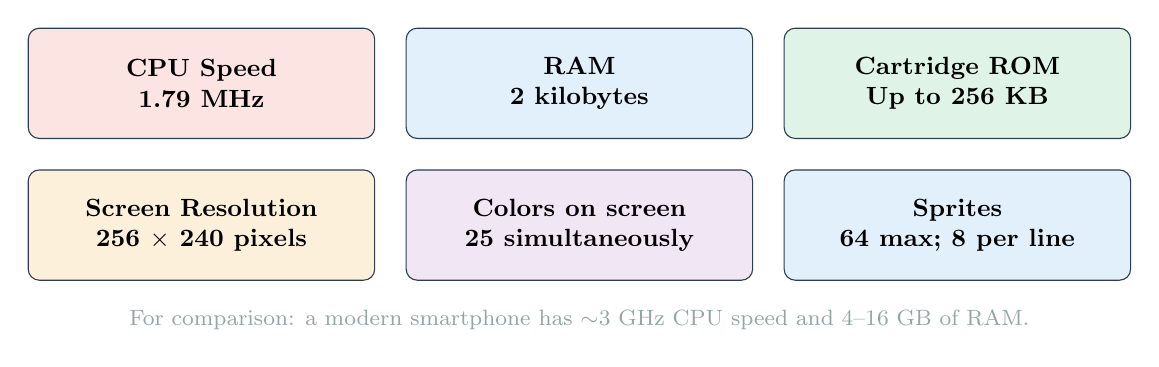
\begin{tikzpicture}[
    spec/.style={rectangle, rounded corners=4pt, draw=csprimary, fill=#1,
                 minimum width=44mm, minimum height=14mm, align=center, font=\small\bfseries},
    label/.style={font=\footnotesize, color=codegray, align=center}
]
\node[spec=cssecondary!15] (cpu) at (0,0)   {CPU Speed\\1.79 MHz};
\node[spec=cstertiary!15]  (ram) at (4.8,0) {RAM\\2 kilobytes};
\node[spec=csaccent!15]    (rom) at (9.6,0) {Cartridge ROM\\Up to 256 KB};
\node[spec=cswarm!15]      (res) at (0,-1.8){Screen Resolution\\256 $\times$ 240 pixels};
\node[spec=codepurple!15]  (col) at (4.8,-1.8){Colors on screen\\25 simultaneously};
\node[spec=cstertiary!15]  (spr) at (9.6,-1.8){Sprites\\64 max; 8 per line};

\node[label] at (4.8,-3.0) {For comparison: a modern smartphone has $\sim$3 GHz CPU speed and 4--16 GB of RAM.};
\end{tikzpicture}
\end{center}

With 2 kilobytes of RAM---enough to store about two pages of text---programmers had no room for abstraction or waste. Every byte was accounted for. Variables were kept in specific memory addresses, hand-chosen for efficiency. Code was written in \keyterm{assembly language}: low-level instructions that map almost directly to the CPU's hardware operations.

\begin{historybox}[Super Mario Bros. (1985): Engineering Marvel in 31 KB]
When Shigeru Miyamoto and Takashi Tezuka designed \textit{Super Mario Bros.}, programmer Toshihiko Nakago had to fit the entire game---world layouts, enemy AI, physics, music, graphics---into 31 kilobytes. His solutions became industry legends:

\textbf{Data compression by reuse:} The underground levels reuse the same tile graphics as the overworld; only the color palette changes. The same enemy sprite is reused with different behaviors. Identical data was never stored twice.

\textbf{Procedural tricks:} Rather than storing every cloud and bush separately, the bush graphic \textit{is} the cloud graphic---just recolored and placed at ground level. Players never noticed.

\textbf{Physics as integers:} Mario's gravity and velocity were stored as simple integers. The ``feel'' of Mario's jump came from carefully tuned integer arithmetic, not floating-point physics simulation.

The result shipped in 31,072 bytes. It sold 40 million copies.
\end{historybox}

\subsection{What Assembly Code Looked Like}

Modern programmers rarely write assembly. But seeing it helps you understand how far the tools have come---and why higher-level abstractions matter.

\begin{asmcode}[6502 Assembly: Moving a Character (NES Era)]
; Move player character right if right button is pressed
; Register A holds button state; each bit is one button
CHECK_RIGHT:
    LDA CONTROLLER_1    ; Load controller input into register A
    AND #%00000001      ; Mask: keep only the rightmost bit
    BEQ NO_RIGHT        ; If zero (not pressed), skip ahead

    LDA PLAYER_X        ; Load player's X position
    CMP #232            ; Are we at the right edge of the screen?
    BCS NO_RIGHT        ; If so, don't move further right
    INC PLAYER_X        ; Otherwise, increment X position by 1

NO_RIGHT:
    RTS                 ; Return from subroutine
\end{asmcode}

Compare this with the equivalent Java:

\begin{javacode}[The Same Logic in Java]
void checkRight(Controller controller, Player player) {
    if (controller.isPressed(Button.RIGHT)) {
        if (player.getX() < 232) {
            player.setX(player.getX() + 1);
        }
    }
}
\end{javacode}

The Java version is longer in lines but far easier to read and reason about. The assembly version is faster and uses less memory---but is nearly impossible to maintain in a large project. Early game developers lived entirely in the assembly world.

\subsection{The First Game Loop}

Even in the NES era, one pattern was already emerging: the \keyterm{game loop}. Every frame, the game had to: read player input, update the game world, and draw everything to the screen. This cycle repeated 60 times per second---forever, until the game ended.

\begin{center}
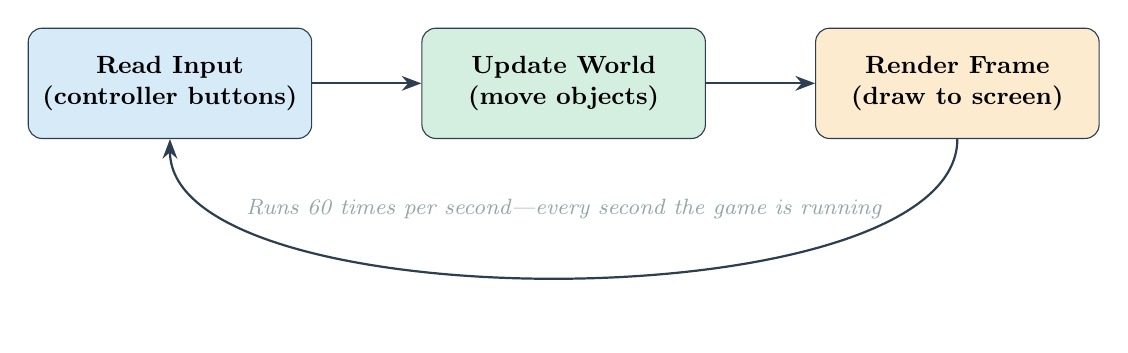
\begin{tikzpicture}[
    box/.style={rectangle, rounded corners=5pt, draw=csprimary, fill=#1,
                minimum width=36mm, minimum height=14mm, align=center, font=\small\bfseries},
    arrow/.style={-{Stealth[length=2.5mm]}, thick, color=csprimary}
]
\node[box=cstertiary!20] (input)  at (0,0)    {Read Input\\(controller buttons)};
\node[box=csaccent!20]   (update) at (5,0)    {Update World\\(move objects)};
\node[box=cswarm!20]     (render) at (10,0)   {Render Frame\\(draw to screen)};

\draw[arrow] (input) -- (update);
\draw[arrow] (update) -- (render);
\draw[arrow] (render.south) to[out=-90, in=-90, looseness=0.6] (input.south);

\node[font=\footnotesize\itshape, color=codegray] at (5,-1.6) {Runs 60 times per second---every second the game is running};
\end{tikzpicture}
\end{center}

This three-phase structure---\textbf{input, update, render}---is the heartbeat of virtually every game ever written, from Pong to \textit{Elden Ring}. We will see it again in Java shortly.

%---------- THE 16-BIT ERA ----------%
\section{The 16-Bit Era: More Room to Breathe (1990--1996)}

\subsection{SNES and Growing Complexity}

The Super Nintendo Entertainment System (SNES, 1990) was a generational leap: more RAM, a faster CPU, more colors, and hardware support for scaling and rotating sprites. But the jump from NES to SNES wasn't just more of the same---it enabled qualitatively richer games, and with them, new programming challenges.

\begin{historybox}[The Legend of Zelda: A Link to the Past (1991)]
\textit{A Link to the Past} is often cited as one of the greatest games ever made. Programmer Yasunari Nishida designed a game world with two parallel dimensions (the Light World and the Dark World), dozens of interconnected rooms, over 100 enemy types, and a complex inventory and progression system.

The key engineering insight: \textbf{data-driven design}. Rather than coding each room individually, Nishida created a format for describing rooms as data---enemy placements, tile arrangements, door connections, event triggers. A small interpreter read this data and constructed each room at runtime. Adding a new room meant creating new data; the code itself rarely needed to change.

This is one of the oldest and most powerful ideas in software engineering: \textbf{separate code from data}. Code handles ``how to do things''; data describes ``what to do.''
\end{historybox}

\begin{historybox}[Super Mario World (1990): Reuse and Extension]
\textit{Super Mario World} launched with the SNES and expanded the Mario formula significantly: Yoshi the dinosaur, capes, secret exits, and a branching world map. Programmer Toshio Iwawaki faced a challenge common in long-running series: how do you build on what came before without starting from scratch?

The answer was \textbf{code reuse}. Core systems from earlier Mario games---the physics model, the enemy behavior framework, the scrolling renderer---were ported and extended. New enemy types were added by defining new behavior data rather than rewriting fundamental code.

\textit{Super Mario World} contains 512 KB of data. Roughly half is level and graphics data---the other half is code that could apply to any Mario game.
\end{historybox}

\subsection{State Machines: Modeling Character Behavior}

One of the most important patterns in game programming---and in software engineering generally---emerged clearly in the 16-bit era: the \keyterm{finite state machine} (FSM).

A state machine describes an object as always being in one of a fixed set of \textbf{states}, with \textbf{transitions} between states triggered by events. Mario, for example, is always in exactly one state at a time.

\begin{center}
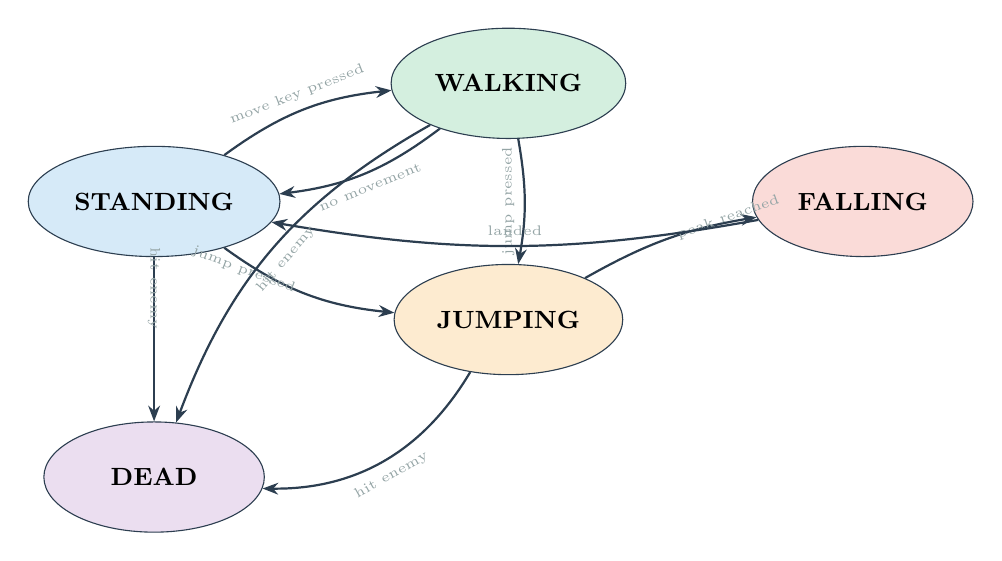
\begin{tikzpicture}[
    state/.style={ellipse, draw=csprimary, fill=#1,
                  minimum width=28mm, minimum height=14mm, align=center, font=\small\bfseries},
    arrow/.style={-{Stealth[length=2mm]}, thick, color=csprimary},
    label/.style={font=\tiny, color=codegray, midway, sloped}
]
\node[state=cstertiary!20]  (idle)   at (0,0)      {STANDING};
\node[state=csaccent!20]    (walk)   at (4.5,1.5)  {WALKING};
\node[state=cswarm!20]      (jump)   at (4.5,-1.5) {JUMPING};
\node[state=cssecondary!20] (fall)   at (9,0)      {FALLING};
\node[state=codepurple!20]  (die)    at (0,-3.5)   {DEAD};

\draw[arrow] (idle) to[bend left=15]  node[label, above] {move key pressed} (walk);
\draw[arrow] (walk) to[bend left=15]  node[label, below] {no movement}      (idle);
\draw[arrow] (idle) to[bend right=15] node[label, left]  {jump pressed}     (jump);
\draw[arrow] (walk) to[bend left=10]  node[label, above] {jump pressed}     (jump);
\draw[arrow] (jump) to[bend left=10]  node[label, right] {peak reached}     (fall);
\draw[arrow] (fall) to[bend left=10]  node[label, above] {landed}           (idle);
\draw[arrow] (idle) to                node[label, left]  {hit enemy}        (die);
\draw[arrow] (walk) to[bend right=20] node[label, below] {hit enemy}        (die);
\draw[arrow] (jump) to[bend left=30]  node[label, below] {hit enemy}        (die);
\end{tikzpicture}
\end{center}

State machines are powerful because they make behavior explicit and exhaustive: you can list every state and every transition. Bugs often come from \textit{missing} transitions---what happens if the player presses jump while already in the FALLING state? A state machine forces you to decide.

In modern Java, a state machine is naturally expressed with an \texttt{enum}:

\begin{javacode}[A State Machine for Mario in Java]
public enum MarioState {
    STANDING, WALKING, JUMPING, FALLING, DEAD
}

public class Mario {
    private MarioState state = MarioState.STANDING;
    private double velocityY = 0;

    public void update(boolean leftHeld, boolean rightHeld,
                       boolean jumpPressed, boolean onGround) {
        switch (state) {
            case STANDING:
                if (leftHeld || rightHeld) state = MarioState.WALKING;
                if (jumpPressed)           state = MarioState.JUMPING;
                break;

            case WALKING:
                if (!leftHeld && !rightHeld) state = MarioState.STANDING;
                if (jumpPressed)             state = MarioState.JUMPING;
                break;

            case JUMPING:
                velocityY -= 0.5;          // gravity pulls down
                if (velocityY < 0)         state = MarioState.FALLING;
                break;

            case FALLING:
                velocityY -= 0.5;
                if (onGround) {
                    velocityY = 0;
                    state = MarioState.STANDING;
                }
                break;

            case DEAD:
                break;                     // no transitions out of DEAD
        }
    }

    public void takeDamage() {
        state = MarioState.DEAD;
    }
}
\end{javacode}

\begin{tipbox}[State Machines Beyond Games]
State machines appear everywhere in software engineering:
\begin{itemize}[itemsep=2pt]
    \item A traffic light cycles through RED $\to$ GREEN $\to$ YELLOW $\to$ RED
    \item A vending machine moves through IDLE $\to$ COIN\_INSERTED $\to$ DISPENSING $\to$ IDLE
    \item A network connection moves through CLOSED $\to$ CONNECTING $\to$ OPEN $\to$ CLOSING
    \item A UI button is NORMAL $\to$ HOVERED $\to$ PRESSED $\to$ NORMAL
\end{itemize}
When you're modeling anything that changes behavior based on what has happened previously, a state machine is often the right tool.
\end{tipbox}

%---------- THE 3D REVOLUTION ----------%
\section{The 3D Revolution: N64 and the C Language (1996--2002)}

\subsection{A New Dimension---and New Complexity}

The Nintendo 64 (1996) introduced 3D gaming to the mainstream, and with it a fundamental change in how games were programmed. Assembly language, already barely adequate for SNES games, was simply not viable for 3D. The math involved---matrix transformations, trigonometry, perspective projection---was too complex to write by hand in low-level code.

The industry switched to \keyterm{C}, a higher-level language that compiled to efficient machine code while allowing programmers to express complex algorithms far more clearly. C is still the dominant language for systems where raw performance is critical; it's the language of the Linux kernel, embedded systems, and many game engines today.

\begin{historybox}[Super Mario 64 (1996): Inventing 3D Game Design]
\textit{Super Mario 64} didn't just port 2D Mario to 3D---it invented much of the vocabulary of 3D game design that is still used today. Programmer Giles Goddard's camera system, Yoshiaki Koizumi's animation framework, and the team's approach to 3D collision detection were all unprecedented.

The challenge of 3D was not just technical but conceptual: how do you let a player navigate a three-dimensional space with a controller that has a limited number of buttons? How do you design a camera that the player doesn't directly control but that always gives a useful view? These ``soft'' engineering problems---designing systems that \textit{feel} right, not just \textit{work} correctly---became as important as the hard technical problems.

\textit{Super Mario 64} contained approximately 3 MB of data and ran at 30 frames per second on hardware without a dedicated GPU in the modern sense. The game's physics, AI, and rendering all competed for the same CPU cycles.
\end{historybox}

\begin{historybox}[The Legend of Zelda: Ocarina of Time (1998)]
\textit{Ocarina of Time} is frequently voted the greatest video game ever made. Its programming team, led by Toru Osawa, built systems that have been studied and imitated for decades:

\textbf{Z-targeting:} A system allowing the player to ``lock on'' to an enemy, automatically orienting the camera and character. This was a novel solution to the 3D combat problem that became a genre standard.

\textbf{Scripted events:} Story moments, NPC dialogue, and environmental triggers were driven by a custom scripting system---a simple programming language that designers could use without writing C code. This separation of ``game logic'' from ``engine code'' is now a universal practice in the industry.

\textbf{Context-sensitive actions:} The same button did different things depending on context: near a ledge, it grabbed the ledge; near an NPC, it talked; near an object, it interacted. This required a carefully engineered system for detecting context and dispatching the right action.
\end{historybox}

\subsection{Objects Arrive in Game Code}

As games grew more complex in the late 1990s and early 2000s, programmers began applying \keyterm{object-oriented programming} (OOP) more systematically. A game world is naturally described in terms of objects: enemies, items, platforms, projectiles, and triggers all have their own data and behavior.

An \keyterm{inheritance hierarchy} became a common organizing structure: all game objects share a base class, with specialized behavior in subclasses.

\begin{javacode}[A Game Object Hierarchy]
// Base class: everything in the game world is a GameObject
public abstract class GameObject {
    protected double x, y;       // Position in the world
    protected double width, height;

    public abstract void update(double deltaTime);
    public abstract void render(Graphics g);

    // Shared utility: axis-aligned bounding box collision
    public boolean collidesWith(GameObject other) {
        return x < other.x + other.width
            && x + width > other.x
            && y < other.y + other.height
            && y + height > other.y;
    }
}

// Characters move and can be hurt
public abstract class Character extends GameObject {
    protected int health;
    protected double velocityX, velocityY;

    public void takeDamage(int amount) {
        health -= amount;
    }

    public boolean isAlive() {
        return health > 0;
    }
}

// Mario is a specific kind of Character
public class Mario extends Character {
    private MarioState state = MarioState.STANDING;

    public Mario(double startX, double startY) {
        x = startX; y = startY;
        width = 16; height = 32;
        health = 1;
    }

    @Override
    public void update(double deltaTime) {
        // Mario-specific update logic (state machine, input, etc.)
    }

    @Override
    public void render(Graphics g) {
        // Draw Mario's current animation frame
    }
}

// Enemies are also Characters
public class Goomba extends Character {
    private double direction = 1.0;   // 1 = right, -1 = left

    @Override
    public void update(double deltaTime) {
        x += direction * 60 * deltaTime;   // Move at 60 px/sec
        // reverse at edges, walls, etc.
    }

    @Override
    public void render(Graphics g) {
        // Draw Goomba sprite
    }
}
\end{javacode}

The hierarchy \texttt{Object $\to$ GameObject $\to$ Character $\to$ Mario/Enemy} lets the rest of the engine work with \texttt{GameObject} references without knowing the specific type---a direct application of \keyterm{polymorphism}. The collision detection method works for any two game objects; rendering and updating work for any list of game objects.

%---------- THE ENGINE ERA ----------%
\section{The Engine Era: Reuse and Large Teams (2002--2012)}

\subsection{What is a Game Engine?}

By the early 2000s, a pattern emerged: the core systems of a game---rendering, physics, audio, input handling, collision detection---were largely the same from one game to the next. Building them from scratch for every project was wasteful.

The solution was the \keyterm{game engine}: a reusable software framework providing common systems, leaving game developers to focus on game-specific content and logic. Engines could be licensed, purchased, or (later) downloaded for free.

\begin{center}
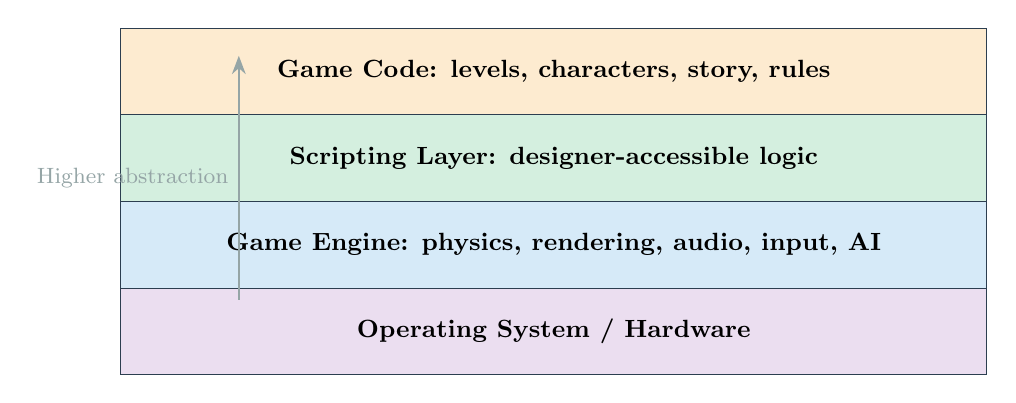
\begin{tikzpicture}[
    layer/.style={rectangle, draw=csprimary, fill=#1,
                  minimum width=110mm, minimum height=11mm,
                  align=center, font=\small\bfseries},
]
\node[layer=cswarm!20]     (game)    at (0, 3.3) {Game Code: levels, characters, story, rules};
\node[layer=csaccent!20]   (script)  at (0, 2.2) {Scripting Layer: designer-accessible logic};
\node[layer=cstertiary!20] (engine)  at (0, 1.1) {Game Engine: physics, rendering, audio, input, AI};
\node[layer=codepurple!20] (os)      at (0, 0.0) {Operating System / Hardware};

\draw[-{Stealth}, thick, color=codegray] (-4.0,0.4) -- (-4.0,3.5)
    node[midway, left, font=\footnotesize, color=codegray] {Higher abstraction};
\end{tikzpicture}
\end{center}

The engine layer is what teams reuse. \textbf{Unreal Engine} (Epic Games, 1998--present) powered games from \textit{Unreal Tournament} to \textit{Fortnite} to \textit{Hogwarts Legacy}. \textbf{Unity} (2005--present) became the dominant engine for independent developers. Entire categories of problems---3D rendering, physics simulation, cross-platform support---were solved once inside the engine and never reimplemented by game developers again.

\begin{historybox}[New Super Mario Bros. (2006) and Series Architecture]
When Nintendo returned Mario to 2D with \textit{New Super Mario Bros.} on the DS, they were drawing on twenty years of accumulated code and design knowledge. The game was built on an internal engine used across Nintendo's handheld titles, with Mario-specific systems layered on top.

The ``feel'' of Mario's jump---the specific parabola, the responsiveness of the controls, the way speed builds up---had been tuned over decades and was preserved as a kind of institutional knowledge: documented physics constants, carefully tested acceleration curves. Even as the hardware changed from NES to SNES to N64 to DS, the \textit{experience} of controlling Mario stayed consistent. This is a software engineering problem as much as a design one: how do you preserve behavior across total platform rewrites?
\end{historybox}

\subsection{Interfaces: Defining What Objects Can Do}

As engines grew larger and teams grew bigger, a new pattern became essential: defining behavior through \keyterm{interfaces} rather than class hierarchies. An interface specifies what an object can do (its \textit{contract}) without specifying how it does it or what else it might be.

\begin{javacode}[Interfaces for Game Object Behaviors]
// Any object that can be updated each frame
public interface Updatable {
    void update(double deltaTime);
}

// Any object that can be drawn to the screen
public interface Renderable {
    void render(Graphics g);
}

// Any object that participates in collision detection
public interface Collidable {
    Rectangle getBounds();
    void onCollision(GameObject other);
}

// Enemies implement all three
public class Koopa extends Character
        implements Updatable, Renderable, Collidable {

    @Override
    public void update(double deltaTime) { /* movement logic */ }

    @Override
    public void render(Graphics g)       { /* draw sprite */    }

    @Override
    public Rectangle getBounds()         { return new Rectangle((int)x, (int)y,
                                                   (int)width, (int)height); }

    @Override
    public void onCollision(GameObject other) {
        if (other instanceof Mario mario) {
            mario.takeDamage(1);
        }
    }
}

// The engine can now manage all game objects through their interfaces,
// without knowing the specific types
public class GameEngine {
    private List<Updatable>  updateables = new ArrayList<>();
    private List<Renderable> renderables = new ArrayList<>();
    private List<Collidable> collidables = new ArrayList<>();

    public void gameLoop(double deltaTime) {
        for (Updatable u  : updateables)  u.update(deltaTime);
        checkCollisions();
        for (Renderable r : renderables)  r.render(screen);
    }
}
\end{javacode}

This design means you can add a new enemy type---a new class you haven't written yet---and the engine will automatically update it, render it, and check its collisions, without changing a single line of engine code. This is the \keyterm{open/closed principle}: the engine is \textit{open} for extension (new types) but \textit{closed} for modification (existing code doesn't change).

\subsection{Version Control and Large Teams}

A team of five programmers could share code by talking to each other. A team of fifty cannot. The engine era coincided with the widespread adoption of \keyterm{version control} in game development.

\begin{debatebox}[The Coordination Problem]
A major game in the 2000s might involve:
\begin{itemize}[itemsep=2pt]
    \item 20--50 programmers writing C++ and scripting code
    \item 50--100 artists creating textures, models, and animations
    \item 10--20 designers building levels and tuning gameplay values
    \item Sound designers, writers, QA testers, and producers
\end{itemize}
All of these people are making changes to the same project simultaneously. Without version control, the last person to save a file ``wins,'' overwriting everyone else's work. \textbf{Git} (and its predecessor, \textbf{Perforce}, which many studios still use) solved this: changes are tracked, merged, and---when conflicts arise---resolved deliberately rather than accidentally.

The lesson for beginning programmers: even working alone, version control protects you from yourself. A bug you introduced last Tuesday is recoverable. Accidentally deleted files are recoverable. The habit of committing often is the cheapest insurance in software development.
\end{debatebox}

%---------- THE INDIE AND MODERN ERA ----------%
\section{The Modern Era: Democratization and Beyond (2012--Present)}

\subsection{Unity and the Indie Revolution}

Something remarkable happened around 2010--2015: the tools for making games became accessible to individuals and tiny teams. \textbf{Unity} (2005, widely adopted ~2010) offered a professional-grade 3D engine for free. Its scripting language, C\#, is closely related to Java---if you know one, you can read the other.

\begin{historybox}[What Unity Changed]
Before Unity, making a 3D game required either licensing an expensive engine or building one from scratch. Unity changed the economics completely: a solo developer or a student could build a 3D game with physics, lighting, and cross-platform support without writing any engine code at all.

The result was an explosion of independent games. \textit{Hollow Knight}, \textit{Cuphead}, \textit{Among Us}, \textit{Escape from Tarkov}, \textit{Rust}, and thousands of other games were built in Unity. The barrier to entry dropped from ``multi-million dollar studio'' to ``person with a laptop and time to learn.''

\textbf{Godot} (open source, free) has emerged as a popular alternative, with a Python-like scripting language and full source code availability. For beginners interested in game development, Godot is an excellent starting point.
\end{historybox}

Unity introduced many beginning programmers to OOP concepts in a game context. Every object in a Unity scene is a \texttt{GameObject}. Behavior is added by attaching \texttt{Component} objects---a pattern called \keyterm{composition over inheritance}.

\begin{javacode}[Unity-Style Component Pattern (Conceptual Java)]
// Instead of deep inheritance (Mario extends Character extends GameObject),
// compose behavior from small, focused components

public class GameObject {
    private List<Component> components = new ArrayList<>();

    public void addComponent(Component c) {
        c.setOwner(this);
        components.add(c);
    }

    public void update(double deltaTime) {
        for (Component c : components) c.update(deltaTime);
    }
}

// Each component handles one responsibility
public class PhysicsComponent extends Component {
    private double velocityX, velocityY;
    public void update(double dt) { /* apply gravity, movement */ }
}

public class SpriteRenderer extends Component {
    private Sprite sprite;
    public void update(double dt) { /* draw sprite at owner's position */ }
}

public class PlayerController extends Component {
    public void update(double dt) { /* read input, drive movement */ }
}

// Building a player: attach the right components
GameObject player = new GameObject();
player.addComponent(new PhysicsComponent());
player.addComponent(new SpriteRenderer(marioSprite));
player.addComponent(new PlayerController());

// Building an enemy: different components, same framework
GameObject goomba = new GameObject();
goomba.addComponent(new PhysicsComponent());
goomba.addComponent(new SpriteRenderer(goombaSprite));
goomba.addComponent(new EnemyAI());
\end{javacode}

This component pattern is now ubiquitous in game engines and increasingly common in other software. Each component has a single responsibility and can be combined freely. Adding a ``bouncy'' physics behavior to any object means adding one component, not modifying the class hierarchy.

\subsection{Modern Zelda: Scale and Systemic Design}

\begin{historybox}[Breath of the Wild (2017): A Systems Approach]
\textit{The Legend of Zelda: Breath of the Wild} is a landmark not just as a game but as an engineering achievement. Its open world contains hundreds of square kilometers, thousands of interactable objects, complex weather and temperature systems, and physics that allows nearly any object to be moved, burned, frozen, or dropped.

The key engineering insight: \textbf{systemic design}. Rather than scripting individual interactions (``when the player throws this specific barrel at this specific enemy, this specific thing happens''), Nintendo built general systems:

\begin{itemize}[itemsep=3pt]
    \item \textbf{Material properties:} Every object has properties like flammability and conductivity. Fire spreads to flammable objects; electricity conducts through metal. These rules apply universally.
    \item \textbf{Physics everywhere:} The same physics engine that moves boulders also moves enemies, items, and Link himself. Players discovered emergent solutions---using physics to solve puzzles in ways Nintendo never anticipated.
    \item \textbf{Emergent behavior:} Because systems interact, behaviors emerge that no designer explicitly programmed. A thunderstorm lights dry grass on fire; the fire spreads uphill on wind; a thermal from the fire lifts Link's paraglider. Three physics/weather rules combine into a moment designers didn't script.
\end{itemize}

The team of $\sim$300 people (large by Nintendo standards, modest by AAA standards) produced a game world that felt hand-crafted because the \textit{rules} were carefully designed---not because every inch was individually authored.
\end{historybox}

\begin{tipbox}[The Systems Lesson for Software Engineers]
``Systemic design'' is game development's term for a general software engineering principle: \textbf{define rules that interact} rather than \textbf{script every case explicitly}.

A fragile approach to discounts in a store system: write special-case code for every promotional combination. A systemic approach: define composable discount rules (percentage off, minimum purchase, category restriction) and let them combine.

The systemic approach requires more upfront design but produces systems that are easier to extend, less prone to bugs, and capable of behavior you didn't anticipate---sometimes in pleasant ways.
\end{tipbox}

%---------- THE FULL GAME LOOP IN JAVA ----------%
\section{Putting It Together: The Game Loop in Java}

Now that we've traced the history, let's see how these patterns come together in modern code. The game loop is the foundation of every game, and writing a simple one is achievable for a beginning Java programmer.

\begin{javacode}[A Complete Simple Game Loop in Java]
public class SimpleGame {
    private boolean running = true;
    private List<GameObject> objects = new ArrayList<>();
    private final long TARGET_FRAME_TIME = 1_000_000_000L / 60; // 60 FPS in ns

    public void run() {
        long lastTime = System.nanoTime();

        while (running) {
            long now = System.nanoTime();
            double deltaTime = (now - lastTime) / 1_000_000_000.0; // seconds
            lastTime = now;

            // --- Phase 1: Input ---
            processInput();

            // --- Phase 2: Update ---
            for (GameObject obj : objects) {
                obj.update(deltaTime);
            }
            checkCollisions();

            // --- Phase 3: Render ---
            render();

            // Cap frame rate: sleep if we finished early
            long elapsed = System.nanoTime() - now;
            if (elapsed < TARGET_FRAME_TIME) {
                try {
                    Thread.sleep((TARGET_FRAME_TIME - elapsed) / 1_000_000);
                } catch (InterruptedException e) {
                    Thread.currentThread().interrupt();
                }
            }
        }
    }

    private void checkCollisions() {
        // Check every pair of collidable objects
        for (int i = 0; i < objects.size(); i++) {
            for (int j = i + 1; j < objects.size(); j++) {
                GameObject a = objects.get(i);
                GameObject b = objects.get(j);
                if (a.collidesWith(b)) {
                    a.onCollision(b);
                    b.onCollision(a);
                }
            }
        }
    }
}
\end{javacode}

Notice \texttt{deltaTime}: rather than moving objects a fixed number of pixels per frame, we multiply by the elapsed time in seconds. This means the game runs at the same logical speed regardless of whether the hardware achieves 30 or 60 frames per second. This technique---\keyterm{delta time}---was invented by game developers and is used throughout real-time software.

\begin{tipbox}[Getting Started with Game Development in Java]
If you want to build a game in Java:
\begin{itemize}[itemsep=4pt]
    \item \textbf{Java2D} is built into the standard library. Use \texttt{JFrame} + \texttt{Canvas} with a \texttt{BufferStrategy} for double-buffered rendering. Good for 2D games; no extra dependencies.
    \item \textbf{LibGDX} is a free Java game framework with 2D/3D support, cross-platform deployment (desktop and Android), and a large community.
    \item \textbf{Godot} uses GDScript (Python-like) or C\#. If you're comfortable with Java syntax, C\# in Godot is very approachable and the engine handles the hard parts.
    \item \textbf{Unity} uses C\#. The free tier is fully functional. Enormous community and documentation. If your goal is making a real game people can play, Unity is the industry standard for independent developers.
\end{itemize}
For a first project: implement a simple Pong clone. It requires a game loop, two paddles (state), a ball (physics), collision detection, and a score counter. Every concept in this case study appears in miniature.
\end{tipbox}

%---------- DISCUSSION QUESTIONS ----------%
\section*{Discussion Questions}

\begin{questionbox}
\begin{enumerate}[leftmargin=*, label=\textcolor{cswarm}{\textbf{\arabic*.}}]
    \item \textbf{Constraints and Creativity:} NES programmers worked with 2KB of RAM and expressed astonishing creativity within those limits. Modern developers have essentially unlimited memory by comparison but still face constraints (performance, development time, team size). How do constraints shape software design? Can too few constraints be a problem?

    \item \textbf{Abstraction Trade-offs:} Moving from assembly to C to OOP to game engines represents a series of trades: control and performance for convenience and expressiveness. Where should a programmer be on this spectrum? Are there situations where a more ``primitive'' approach is the right choice?

    \item \textbf{The State Machine Pattern:} We modeled Mario's behavior as a state machine. Think of a system you use every day---a vending machine, a traffic light, an elevator, a shopping cart. Draw (or describe) its states and transitions. Are there edge cases the design needs to handle that aren't obvious at first?

    \item \textbf{Inheritance vs.\ Composition:} We saw two approaches to organizing game objects: inheritance hierarchies (\texttt{Mario extends Character extends GameObject}) and composition (\texttt{GameObject} + attached \texttt{Component} objects). What are the advantages and disadvantages of each? When might you prefer one over the other?

    \item \textbf{Systemic vs.\ Scripted Design:} \textit{Breath of the Wild} achieved its rich world through systemic rules rather than hand-scripted events. Can you think of a software system outside of games that would benefit from a more systemic approach? What rules would you define, and what emergent behaviors might result?
\end{enumerate}
\end{questionbox}

%---------- GLOSSARY ----------%
\section*{Key Terms}

\begin{glossarybox}
\begin{description}[leftmargin=!, labelwidth=3.6cm, font=\bfseries\color{cssecondary}]
    \item[Assembly Language] A low-level programming language with a close correspondence to machine instructions; used for NES and early arcade game programming where performance and memory efficiency were critical.

    \item[Component Pattern] A design approach where behavior is composed from small, focused components attached to an object at runtime, rather than inherited from a class hierarchy.

    \item[Data-Driven Design] Separating code (which describes \textit{how} to do things) from data (which describes \textit{what} to do), so that content can be changed without modifying the program itself.

    \item[Delta Time] The elapsed time since the last frame, used to scale movement and physics so that game speed is consistent regardless of frame rate.

    \item[Finite State Machine] A model of behavior where an object is always in one of a defined set of states, with transitions between states triggered by specific events or conditions.

    \item[Game Engine] A reusable software framework providing core game systems (rendering, physics, audio, input) that developers build on top of rather than reimplementing for each game.

    \item[Game Loop] The central pattern of game programming: a loop that continuously reads input, updates the game world, and renders the result, repeating dozens of times per second.

    \item[Interface] A Java construct that defines a set of method signatures (a contract) that a class promises to implement, enabling polymorphic behavior without requiring a shared base class.

    \item[Open/Closed Principle] A design principle stating that software should be open for extension (new types can be added) but closed for modification (existing code need not change).

    \item[Polymorphism] The ability to treat objects of different types uniformly through a common interface or base class, enabling code to work with types not yet written.

    \item[Scripting Layer] A higher-level language or system used by game designers to write game logic without working directly in the engine's main programming language.

    \item[Systemic Design] Building game worlds (or software systems) through composable rules that interact, rather than scripting every specific scenario, enabling emergent behavior.

    \item[Version Control] A system (such as Git) that tracks changes to code and assets over time, enabling teams to collaborate without overwriting each other's work and allowing any change to be reversed.
\end{description}
\end{glossarybox}

\vspace{5mm}

%---------- FOOTER ----------%
\begin{center}
\textcolor{csprimary}{\rule{0.6\textwidth}{0.5pt}}\\[3mm]
{\small\textcolor{gray}{This case study is part of the Open Educational Resources for \cscourse.\\
Licensed under Creative Commons Attribution 4.0 (CC BY 4.0).}}
\end{center}

\end{document}
